\begin{figure}[ht!]
    \begin{subfigure}{.5\textwidth}
    \centering
    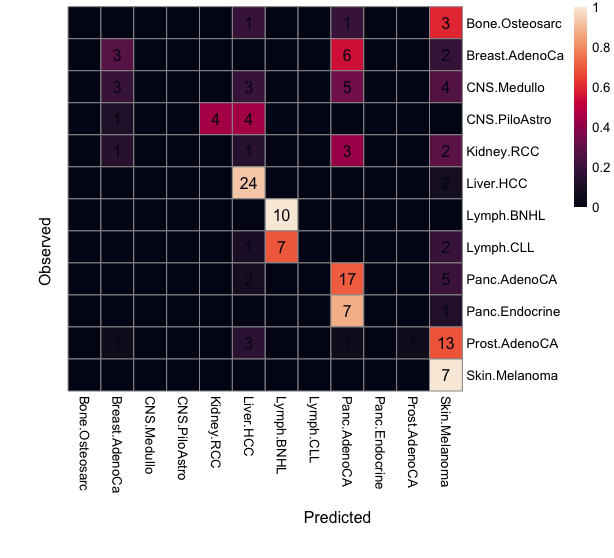
\includegraphics[width=\textwidth,height=0.9\textwidth]{graphics/confusion_matrix_bins_euclidean.png}
    \caption{Bin/Euclidean}
    \label{fig:confusion_bin_euclidean}
    \end{subfigure}
    ~
    \begin{subfigure}{.5\textwidth}
    \centering
    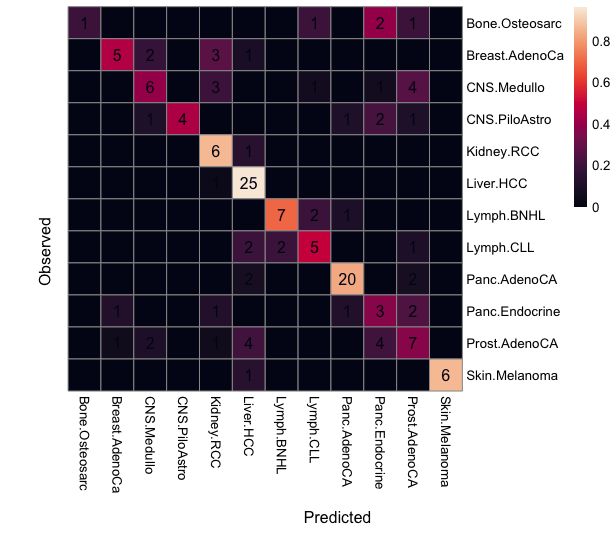
\includegraphics[width=\textwidth,height=0.9\textwidth]{graphics/confusion_matrix_smooth_euclidean.png}
    \caption{Smooth/Euclidean}
    \label{fig:confusion_smooth_euclidean}
    \end{subfigure} \\
    \vspace{0.5cm}
    
    \begin{subfigure}{\textwidth}
    \centering
    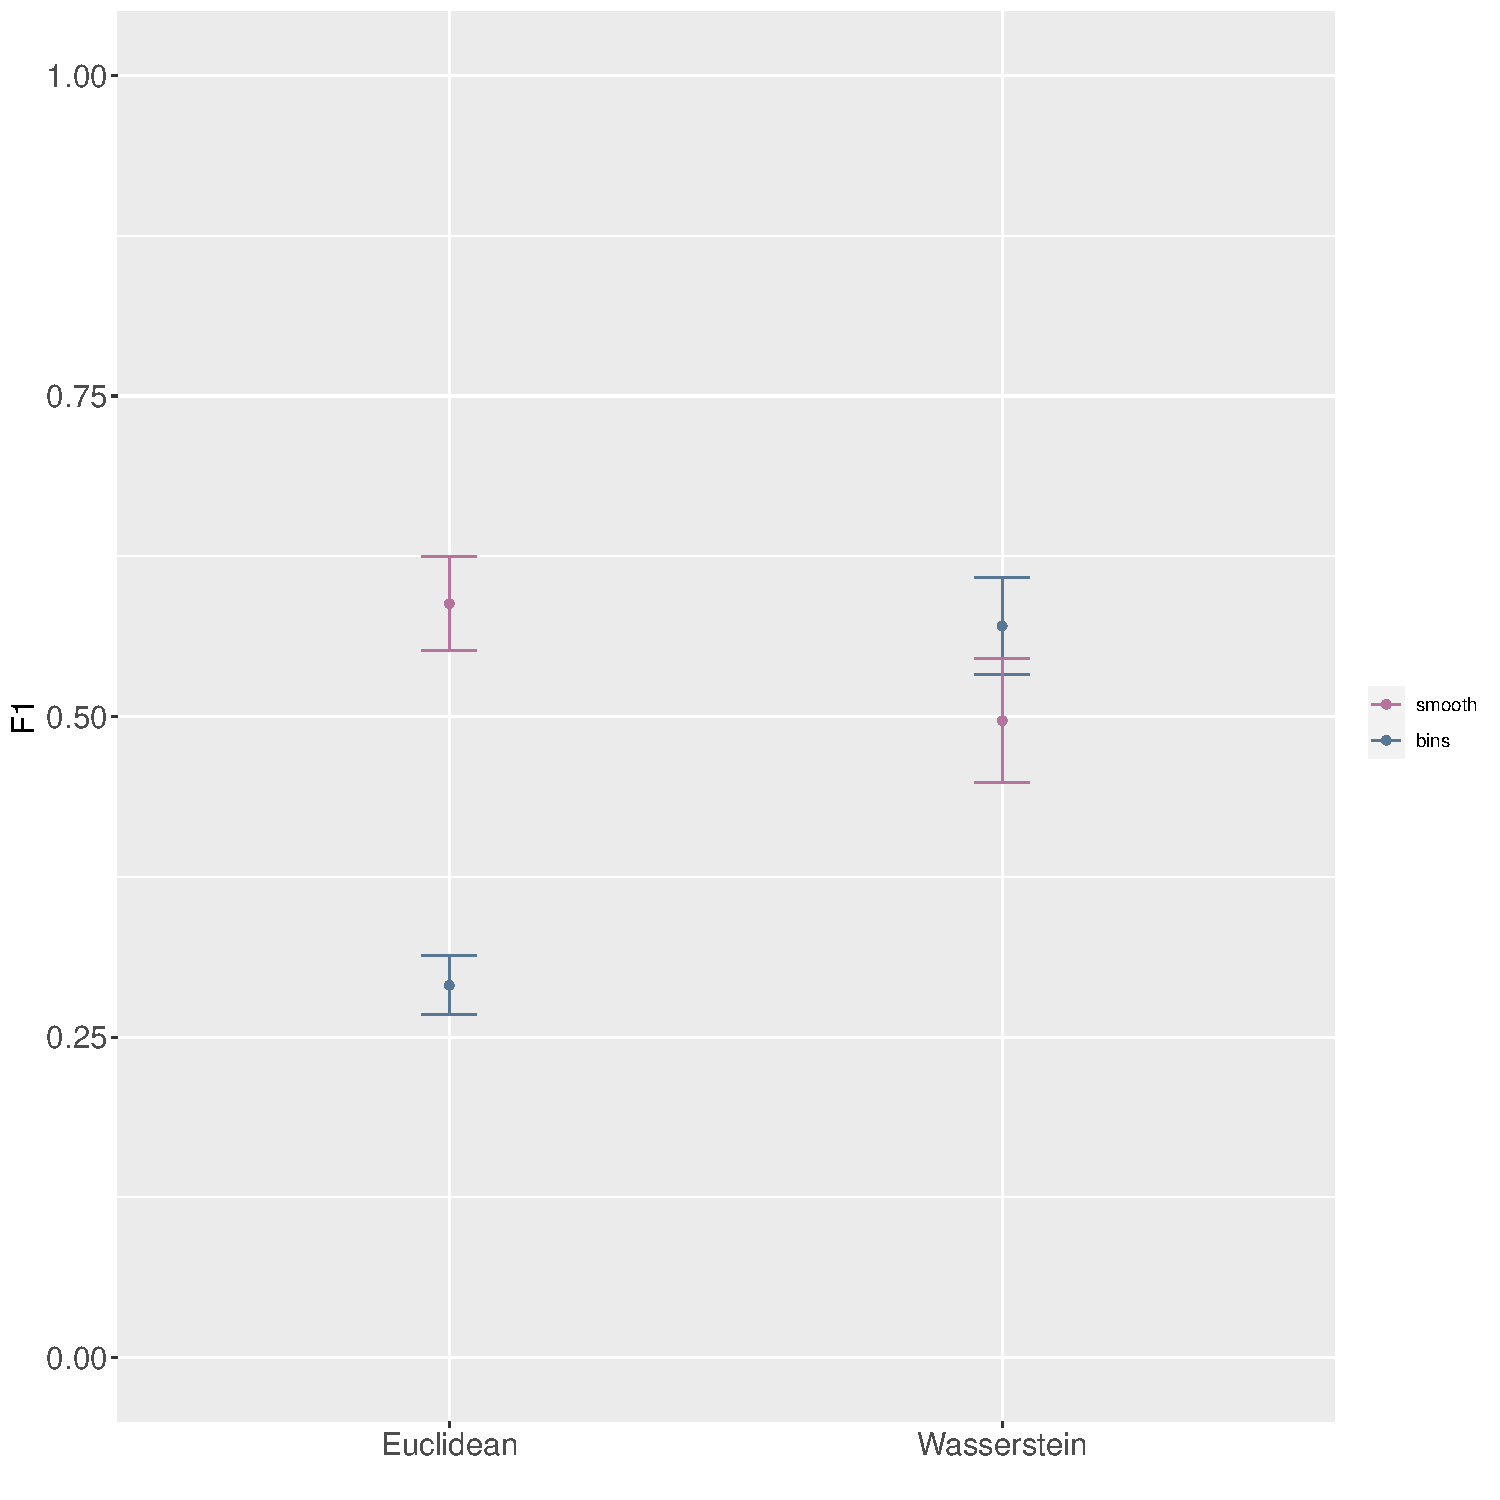
\includegraphics[scale=0.8]{graphics/f1_gle.pdf}
    \caption{F1 summary}
    \label{fig:f1_gle}
    \end{subfigure}
    \vspace{0.5cm}
    
    \caption{\textbf{The smooth representation with the Euclidean distance was the most accurate in predicting cancers.} For each combination of representation/metric, I iterated the training procedures of the KNN classifier 10 times. The performance of the classifier was computed based on a previously held out test data set and reported as confusion matrices and $F1$'s. Here, a representative confusion matrix, coloured by the percentage of predicted values over row total, is shown for (a) Bin/Euclidean, (b) Smooth/Euclidean. The confusion matrices for the Wasserstein distance can be found in Figure \ref{fig:apdx_ml_gle}. Panel (c) shows the means of $F1$ for all representations/measures out of all iterations, the error bars are the standard errors for the iterated $F1$'s.}
    \label{fig:ml_gle}
\end{figure}